\subsection*{JUnit \& EMMA}

\begin{Frame}{Unit Testing in Practice}
  \begin{itemize}
    \item Most methodologies for unit testing, the rest rather ad-hoc (but see later).
    \item Unit testing often done by the programmer.
  \end{itemize}

  \inhead{Popular Procedure for Self-testing}
  \begin{enumerate}
    \item Use a black-box technique to generate\\
      a first set of test cases.
    \item Use a tool to compute the degree of coverage and\\
      the statements/edges/conditions/multiple conditions\\
      not yet covered.
    \item Add new test cases to provide full coverage or\\
      a degree of coverage considered adequate.
    \item The module can only be delivered for integration\\
      together with the (successfully passed) test cases.
  \end{enumerate}
\end{Frame}



\subsubsection*{JUnit}

\begin{frame}{JUnit}
  \begin{itemize}
    \item Unit testing framework for Java
    \item Developed by Erich Gamma and Kent Beck
    \item Current version: JUnit 5.x 
    \item Download: Comes with Eclipse or at \href{http://www.junit.org}{www.junit.org}
    \item Goal: Simplify the definition of test cases (as Java code) and the execution of test cases for Java.
  \end{itemize} 
\end{frame}

\begin{Frame}[fragile]{Simple Test Case (Beck \& Gamma)}
  \begin{itemize}
    \item Annotate a method with \lstinline[language=Java]-@org.junit.Test-.
    \item When you want to check a value
      \begin{lstlisting}[language=java,gobble=8]
        import static org.junit.Assert.*;
      \end{lstlisting}
    \item Call \lstinline[language=Java]-assertTrue();- and pass a boolean that is true if the test succeeds.
  \end{itemize}

  \xxx

  \begin{lstlisting}[language=java,gobble=4]
    @Test
    public void simpleAdd() {
      Money m12CHF = new Money(12, "CHF"); 
      Money m14CHF = new Money(14, "CHF"); 
      Money expected = new Money(26, "CHF"); 
      Money result = m12CHF.add(m14CHF); 
      assertTrue("Money should add up",
        expected.equals(result));
    }
  \end{lstlisting}
\end{Frame}

\begin{Frame}[allowframebreaks,fragile]{Other Assertion Statements}
  Without any assertion a test always passes.

  \xxx

  \begin{lstlisting}[language=Java,gobble=4]
    fail(String message);
  \end{lstlisting}
  Let the test case fail with the given message.

  \xxx

  \begin{lstlisting}[language=Java,gobble=4]
    assertEquals(String message,
      expected, actual);
  \end{lstlisting}

  Test if the values are the same. Note: for arrays the reference is checked not the content of the arrays.

  \xxx

  \begin{lstlisting}[language=Java,gobble=4]
    assertArrayEquals(String message,
      expecteds, actuals);
  \end{lstlisting}

  Test if the given arrays contain the same values.

  \framebreak

  \begin{lstlisting}[language=Java,gobble=4]
    assertEquals(String message,
      expected, actual, tolerance);
  \end{lstlisting}

  Usage for float and double; the tolerance are the number of decimals which must be the same.

  \xxx

  \begin{lstlisting}[language=Java,gobble=4]
    assertNull(String message, object);
  \end{lstlisting}

  Test of an object reference is null.

  \xxx

  \begin{lstlisting}[language=Java,gobble=4]
    assertSame(String message,
      expected, actual);
  \end{lstlisting}

  Test if the given object references point to the some object.

  \framebreak

  \begin{lstlisting}[language=Java,gobble=4]
    assertTrue(String message,
      boolean condition);
  \end{lstlisting}

  Test if the boolean condition holds. Avoid usage if any other assertion is more specific.
\end{Frame}

\begin{Frame}{Fixture (Beck \& Gamma)}
  How to write many test cases for operating within the same
    environment/setup/\alert{fixture}?
  \begin{enumerate}
    \item Add a field for each part of the fixture.
    \item Annotate a method with \lstinline[language=java]-@org.junit.Before- and initialize the variables in that method.
    \item Annotate a method with \lstinline[language=java]-@org.junit.After- to release any permanent resources you allocated in setup.
  \end{enumerate}
\end{Frame}

\begin{Frame}[fragile]{Fixture (Beck \& Gamma)}{Example}
  \begin{lstlisting}[language=java,gobble=4]
    public class MoneyTest { 
      private Money f12CHF; 
      private Money f14CHF; 
      private Money f28USD; 
    
      @Before
      public void setUp() { 
        f12CHF = new Money(12, "CHF"); 
        f14CHF = new Money(14, "CHF"); 
        f28USD = new Money(28, "USD"); 
      }
    }
  \end{lstlisting}
\end{Frame}

\begin{Frame}[fragile]{Running Tests (Beck \& Gamma)}
  \begin{itemize}
    \item Run from a Java program:
      \begin{lstlisting}[language=java,gobble=8]
        org.junit.runner.JUnitCore.
          runClasses(TestClass1.class,...);
      \end{lstlisting}
    \item Run from the command line:
      \begin{lstlisting}[language={},gobble=8]
        java org.junit.runner.JUnitCore \
          TestClass1 [...other test classes...]
      \end{lstlisting}
      with both your test class and junit on the classpath.
    \item Run from the command line using maven:
      \begin{lstlisting}[language={},gobble=8]
        mvn test -Dtest=TestClass1
      \end{lstlisting}
      Leave out the \lstinline[language={}]=-Dtest= option to run all tests.
  \end{itemize}
\end{Frame}

\begin{Frame}[fragile]{Expected Exception (Beck \& Gamma)}
  \begin{lstlisting}[language=java,gobble=4]
    new ArrayList<Object>().get(0);
  \end{lstlisting}
  should throw \lstinline[language=java]-IndexOutOfBoundsException-

  \xxx

  \begin{lstlisting}[language=java,gobble=4]
    @Test(expected=
      IndexOutOfBoundsException.class)
    public void empty() { 
      new ArrayList<Object>().get(0); 
    }
  \end{lstlisting}
\end{Frame}

\begin{Frame}{Other Annotations}
  \begin{itemize}
    \item \lstinline[language=java]-@BeforeClass- performs the method before the start of all tests. This can be used to perform time intensive activities, e.g. connect to a database.
    \item \lstinline[language=java]-@AfterClass- performs the method after all tests have finished. This can be used to perform clean-up activities, e.g. disconnect from a database.
    \item \lstinline[language=java]-@Ignore- ignores the test method, e.g. useful if the underlying code has been changed and the test has not yet been adapted or if the runtime of this test is just to long to be included.
    \item \lstinline[language=java]-@Test(timeout=100)- fails if the method takes longer then 100 milliseconds.
  \end{itemize}
\end{Frame}

\begin{frame}{Testing Frameworks}
Testing frameworks exist for most programming languages, for example
\begin{itemize}
	\item JUnit for Java
	\item Scalatest for Scala
	\item Check, cUnit and many more for C
	\item ...
\end{itemize}
\end{frame}

\subsubsection*{Checking Coverage with EMMA}

\begin{frame}[fragile]{Checking Coverage with EMMA}
  \begin{itemize}
    \item EMMA: \href{http://emma.sourceforge.net/}{emma.sourceforge.net}
    \item Run EMMA on the command line:
      \begin{lstlisting}[language={},gobble=8]
        java -cp emma.jar emmarun -jar \
          YourApp.jar
      \end{lstlisting}
      Insert \texttt{emmarun} between the JVM and your application.
    \item Run EMMA in Eclipse:\\
      Install EclEmma through the Eclipse Marketplace.
  \end{itemize}
\end{frame}

\begin{Frame}{Checking Coverage with EMMA}{Install EclEmma in Eclipse}
  \begin{center}
	  \only<presentation>{%
	    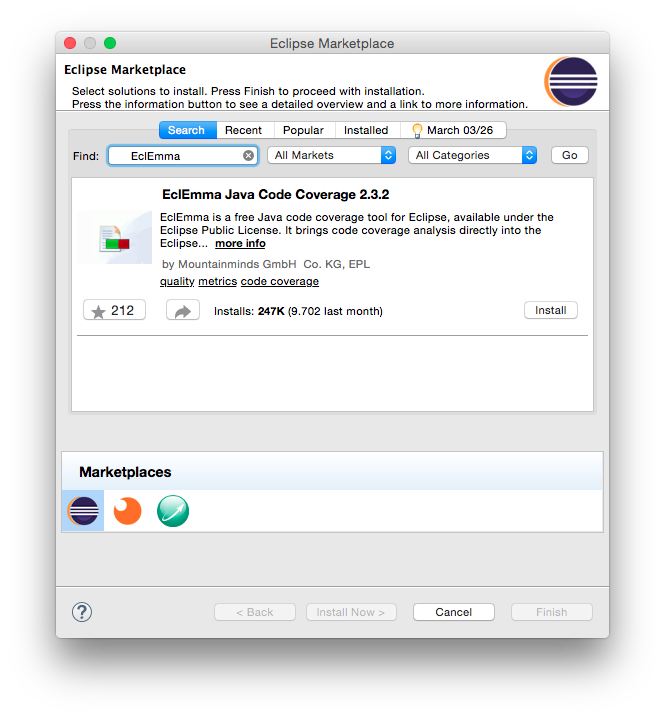
\includegraphics[height=.9\textheight]{content/chapter_testing/black+white/emma-eclipse-marketplace}
    }%
    \only<article>{%
	    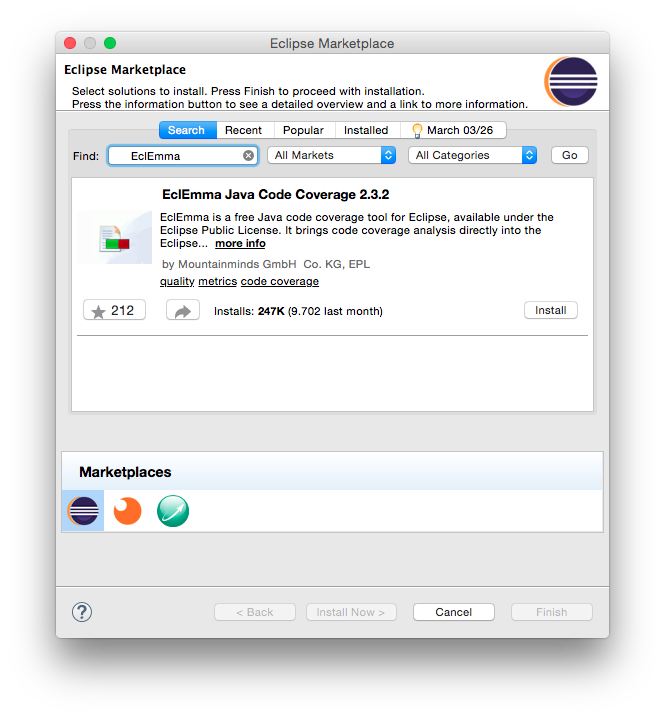
\includegraphics[width=\textwidth]{content/chapter_testing/black+white/emma-eclipse-marketplace}
    }%
  \end{center}
\end{Frame}

\subsubsection*{Triangle Example}

\begin{frame}{Recall the Triangle Exercise (Myers)}
  \begin{itemize}
    \item Input: three integer values\\
      representing lengths of the sides of a triangle.
    \item Output: \texttt{scalene}, \texttt{isosceles}, or \texttt{equilateral}
  \end{itemize}

  \xxx

  \hfill
  \shortstack{
    \tikz[auto,scale=.5]{
      \draw[draw=maincolor, thick]
        (0,0) -- node {4} ++(-4,0) -- node{3} ++(0,3) coordinate (last) -- cycle;
      \path (last) -- node{5} (0,0);}\\
    \texttt{scalene}\strut\\
    \scriptsize (unregelmäßig)
  }
  \hfill
  \shortstack{
    \tikz[auto,scale=.5]{
      \draw[draw=maincolor, thick]
        (0,0) -- node {3} ++(2,2.2361) -- node{3} ++(2,-2.2361) coordinate (last) -- cycle;
      \path (last) -- node{4} (0,0);}\\
    \texttt{isosceles}\strut\\
    \scriptsize (gleichschenklig)
  }
  \hfill
  \shortstack{
    \tikz[auto,scale=.5]{
      \draw[draw=maincolor, thick]
        (0,0) -- node {4} ++(2,3.4641) -- node{4} ++(2,-3.4641) coordinate (last) -- cycle;
      \path (last) -- node{4} (0,0);}\\
    \texttt{equilateral}\strut\\
    \scriptsize (gleichseitig)
  }
  \hfill\strut
\end{frame}

\begin{Frame}[fragile]{Write Java Skeleton}
  \begin{lstlisting}[language=java,gobble=4,basicstyle=\ttfamily\footnotesize]
    public class Triangle {
      public static enum Type {
        SCALENE, ISOSCELES, EQUILITERAL, INVALID;
      }
      
      public static Type getType(int a, int b, int c) {
        // TODO: implement
        throw new UnsupportedOperationException();
      }
    }
  \end{lstlisting}
\end{Frame}

\begin{Frame}[fragile,allowframebreaks]{Write Test Cases}
  \begin{lstlisting}[language=java,gobble=4,basicstyle=\ttfamily\footnotesize]
    @Test
    public void validScalene() {
      assertEquals(SCALENE, getType(2, 3, 4));
    }
    @Test
    public void validEquiliteral() {
      assertEquals(EQUILITERAL, getType(3, 3, 3));
    }
    @Test
    public void validIsoscelesAB() {
      assertEquals(ISOSCELES, getType(3, 3, 5));
    }
    @Test
    public void validIsoscelesAC() {
      assertEquals(ISOSCELES, getType(3, 5, 3));
    }
    @Test
    public void validIsoscelesBC() {
      assertEquals(ISOSCELES, getType(5, 3, 3));
    }
  \end{lstlisting}

  \framebreak

  \begin{lstlisting}[language=java,gobble=4,basicstyle=\ttfamily\footnotesize]
    @Test
    public void invalidZero() {
      assertEquals(INVALID, getType(0, 3, 3));
    }
    @Test
    public void invalidNegative() {
      assertEquals(INVALID, getType(-2, 3, 4));
    }
    @Test
    public void invalidNoAreaAB() {
      assertEquals(INVALID, getType(3, 3, 6));
    }
    @Test
    public void invalidNoAreaAC() {
      assertEquals(INVALID, getType(3, 6, 3));
    }
    @Test
    public void invalidNoAreaBC() {
      assertEquals(INVALID, getType(6, 3, 3));
    }
  \end{lstlisting}

	\framebreak

  \begin{lstlisting}[language=java,gobble=4,basicstyle=\ttfamily\footnotesize]
    @Test
    public void invalidTooLongA() {
      assertEquals(INVALID, getType(4, 2, 1));
    }
    @Test
    public void invalidTooLongB() {
      assertEquals(INVALID, getType(2, 4, 1));
    }
    @Test
    public void invalidTooLongC() {
      assertEquals(INVALID, getType(1, 2, 4));
    }
    @Test
    public void invalidZeros() {
      assertEquals(INVALID, getType(0, 0, 0));
    }
  \end{lstlisting}
\end{Frame}

\begin{Frame}{Run Test Cases}
  \begin{center}
    \only<presentation>{%
	    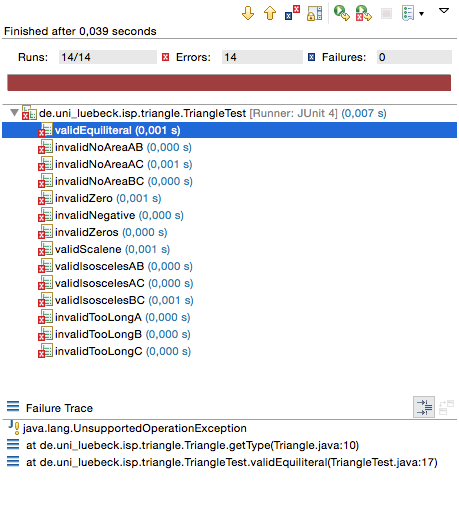
\includegraphics[height=.9\textheight]{content/chapter_testing/black+white/junit-fail}
    }%
    \only<article>{%
	    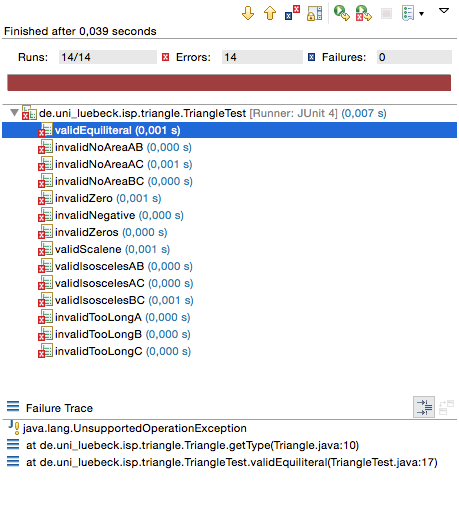
\includegraphics[width=\textwidth]{content/chapter_testing/black+white/junit-fail}
    }%
  \end{center}
\end{Frame}

\begin{Frame}[fragile]{Implement Method}
  \begin{lstlisting}[language=java,gobble=4,basicstyle=\ttfamily\footnotesize]
    public static Type getType(int a, int b, int c) {
      if (a <= 0 || b <= 0)
        return INVALID;
      if (abs(a) + abs(b) <= abs(c))
        return INVALID;
      if (abs(a) + abs(c) <= abs(b))
        return INVALID;
      if (abs(b) + abs(c) <= abs(a))
        return INVALID;
      if (a == b && b == c)
        return EQUILITERAL;
      if (a == b || b == c || a == c)
        return ISOSCELES;
      return SCALENE;
    }
  \end{lstlisting}
\end{Frame}

\begin{Frame}{Run Test Cases Again}
  \begin{center}
	  \only<presentation>{%
	    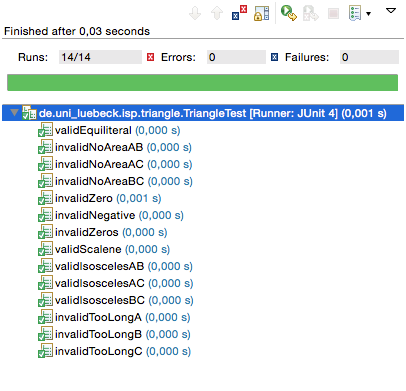
\includegraphics[height=.9\textheight]{content/chapter_testing/black+white/junit-pass}
    }%
    \only<article>{%
    	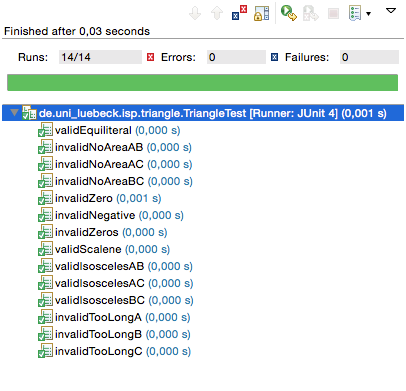
\includegraphics[width=\textwidth]{content/chapter_testing/black+white/junit-pass}
    }%
  \end{center}
\end{Frame}

\begin{Frame}{Run Coverage}
  \begin{center}
    \only<presentation>{%
	    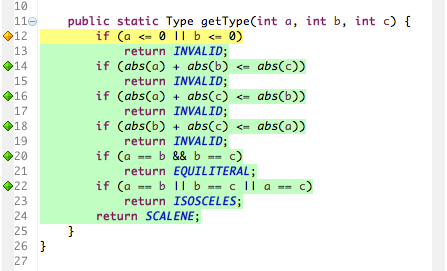
\includegraphics[width=.9\textheight]{content/chapter_testing/black+white/emma-fail}
    }%
    \only<article>{%
      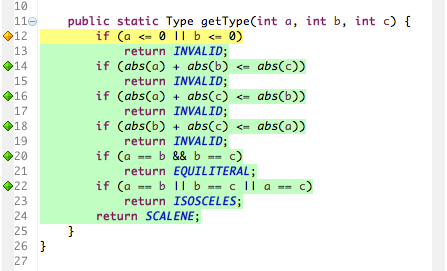
\includegraphics[width=\textwidth]{content/chapter_testing/black+white/emma-fail}
    }%
  \end{center}

  \xxx

  Negative values not completely tested.
\end{Frame}

\begin{Frame}[fragile]{Add More Test Cases}
  \begin{lstlisting}[language=java,gobble=4,basicstyle=\ttfamily\footnotesize]
    @Test
    public void invalidNegativeA() {
      assertEquals(INVALID, getType(-2, 3, 4));
    }
    @Test
    public void invalidNegativeB() {
      assertEquals(INVALID, getType(3, -2, 4));
    }
    @Test
    public void invalidNegativeC() {
      assertEquals(INVALID, getType(3, 4, -2));
    }
  \end{lstlisting}

  \xxx

  Only test case \lstinline[language=java]-invalidNegativeA- was already present.
\end{Frame}

\begin{Frame}{Run Test Cases Again}
  \centerline{
    \only<presentation>{%
      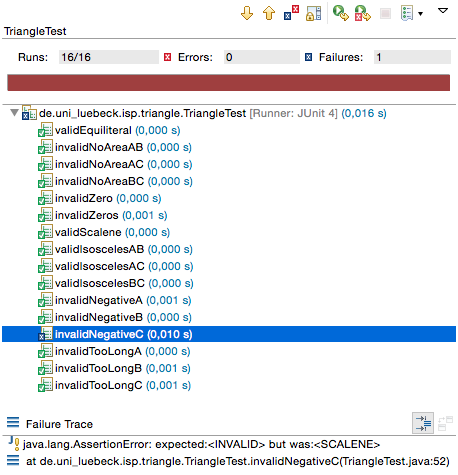
\includegraphics[height=.8\textheight]{content/chapter_testing/black+white/junit-bug}
    }%
    \only<article>{%
      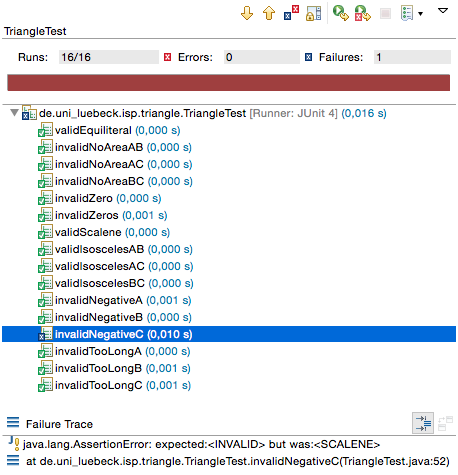
\includegraphics[width=\textwidth]{content/chapter_testing/black+white/junit-bug}
    }%
  }

  We found a bug.
\end{Frame}

\begin{Frame}[fragile]{Fix Implemented Method}
  \begin{lstlisting}[language=java,gobble=4,escapechar=/]
    if (a <= 0 || b <= 0/\alert{\texttt{ || c <= 0}}/)
      return INVALID;
  \end{lstlisting}

  \xxx

  \begin{LARGE}
    Now the test cases pass and\\
    cover the whole implementation.
  \end{LARGE}
\end{Frame}

